\documentclass[11pt]{article}

% basic packages
\usepackage[margin=1in]{geometry}
\usepackage[pdftex]{graphicx}
\usepackage{amsmath,amssymb,amsthm}
\usepackage{custom}
\usepackage{lipsum}

\usepackage{xcolor}
\usepackage{tikz-cd}

\usepackage[most]{tcolorbox}
\usepackage{xcolor}
\usepackage{mdframed}
\usepackage{calligra}


% page formatting
\usepackage{fancyhdr}
\pagestyle{fancy}

\renewcommand{\sectionmark}[1]{\markright{\textsf{\arabic{section}. #1}}}
\renewcommand{\subsectionmark}[1]{}
\lhead{\textbf{\thepage} \ \ \nouppercase{\rightmark}}
\chead{}
\rhead{}
\lfoot{}
\cfoot{}
\rfoot{}
\setlength{\headheight}{14pt}

\linespread{1.03} % give a little extra room
\setlength{\parindent}{0.2in} % reduce paragraph indent a bit
\setcounter{secnumdepth}{2} % no numbered subsubsections
\setcounter{tocdepth}{2} % no subsubsections in ToC

\DeclareMathAlphabet{\mathcalligra}{T1}{calligra}{m}{n}
\DeclareFontShape{T1}{calligra}{m}{n}{<->s*[2.2]callig15}{}
\newcommand{\scriptr}{\mathcalligra{r}\,}
\newcommand{\boldscriptr}{\pmb{\mathcalligra{r}}\,}


%%%%%%%%%%%%%%%%%%%%%%%%%%%%%%%%%%%%%%%%%%%%%%%%%%%%%%%%%%%%%%%%%
% CUSTOM BOXES AND STUFF
\newtcolorbox{redbox}{colback=red!5!white,colframe=red!75!black, breakable}
\newtcolorbox{bluebox}{colback=blue!5!white,colframe=blue!75!black, breakable}

\definecolor{lightblue}{RGB}{173,216,230} % Light blue color
\definecolor{darkblue}{RGB}{0,0,139} % Dark blue color

% Define the custom proof environment
\newtcolorbox{ex}[2][Example]{
  colback=red!5!white, % Light blue background
  colframe=red!75!black, % Darker blue border
  coltitle=white, % Title color
  fonttitle=\bfseries, % Title font style
  title={{#2}},
  arc=1mm, % Rounded corners with 4mm radius,
  boxrule=0.5mm,
  left=2mm, right=2mm, top=2mm, bottom=2mm, % Padding inside the box
  breakable, % Allow box to be broken across pages
  before=\vspace{10pt}, % Padding above the box
  after=\vspace{10pt}, % Padding below the box
  before upper={\parindent15pt} % Ensure indentation
}

% Define the custom proof environment
\newtcolorbox{defn}[2][Definition]{
  colback=blue!5!white, % Light blue background
  colframe=blue!75!black, % Darker blue border
  coltitle=white, % Title color
  fonttitle=\bfseries, % Title font style
  title={{#2}},
  arc=1mm, % Rounded corners with 4mm radius,
  boxrule=0.5mm,
  left=2mm, right=2mm, top=2mm, bottom=2mm, % Padding inside the box
  breakable, % Allow box to be broken across pages
  before=\vspace{10pt}, % Padding above the box
  after=\vspace{10pt}, % Padding below the box
  before upper={\parindent15pt} % Ensure indentation
}


%%%%%%%%%%%%%%%%%%%%%%%%%%%%%%%%%%%%%%%%%%%%%%%%%%%%%%%%%%%%%%%%%


\begin{document}

% make title page
\thispagestyle{empty}
\bigskip \
\vspace{0.1cm}

\begin{center}
{\fontsize{22}{22} \selectfont (Instructor: James Analytis)}
\vskip 16pt
{\fontsize{36}{36} \selectfont \bf \sffamily Physics 141B: Introduction to Solid State II Notes}
\vskip 24pt
{\fontsize{18}{18} \selectfont \rmfamily Keshav Balwant Deoskar} 
\vskip 6pt
{\fontsize{14}{14} \selectfont \ttfamily kdeoskar@berkeley.edu} 
\vskip 24pt
\end{center} These are some notes taken from UC Berkeley's Physics 141B during the Fall '24 session, taught by James Analytis. This template is based heavily off of the one produced by \href{https://knzhou.github.io/}{Kevin Zhou}.

% \microtoc
\tableofcontents 


%%%%%%%%%%%%%%%%%%%%%%%%%%%%%%%%%%%%%%%%%%%%%%%%
\pagebreak
\section{January 22, 2025:}
%%%%%%%%%%%%%%%%%%%%%%%%%%%%%%%%%%%%%%%%%%%%%%%%

Office Hours Fri 1-2pm after Lecture.\\
Syllabus: 
\begin{itemize}
  \item Topology: (6-7 weeks)
  \begin{itemize}
    \item Su-Shrieffer-Heeger Model
    \item Berry's Phase and its application to Graphene
    \item Haldane Model
    \item Topological Insulators
  \end{itemize}

  \item Superconductivity: (3-4 weeks)
  \begin{itemize}
    \item Overview and Two-fluid Model
    \item Cooper pairing
    \item Bardeen, Cooper, Schrieffer (BCS) Model
    \item Josephson Effect
  \end{itemize}

  \item If we have time, Magnetism: 
  \begin{itemize}
    \item Phenomenology, Ferromagnets and Antiferromagnets
    \item Direct-exchange and Super-exchange
    \item Mean-field Model
  \end{itemize}
\end{itemize}

\vskip 1cm
\subsection{Review: The Tight Binding model}
Consider a 1D Chain of $N$ sites with 1 orbital per site, and consider a unit cell with 1 site per cell defined as in the picture below:
\begin{center}
  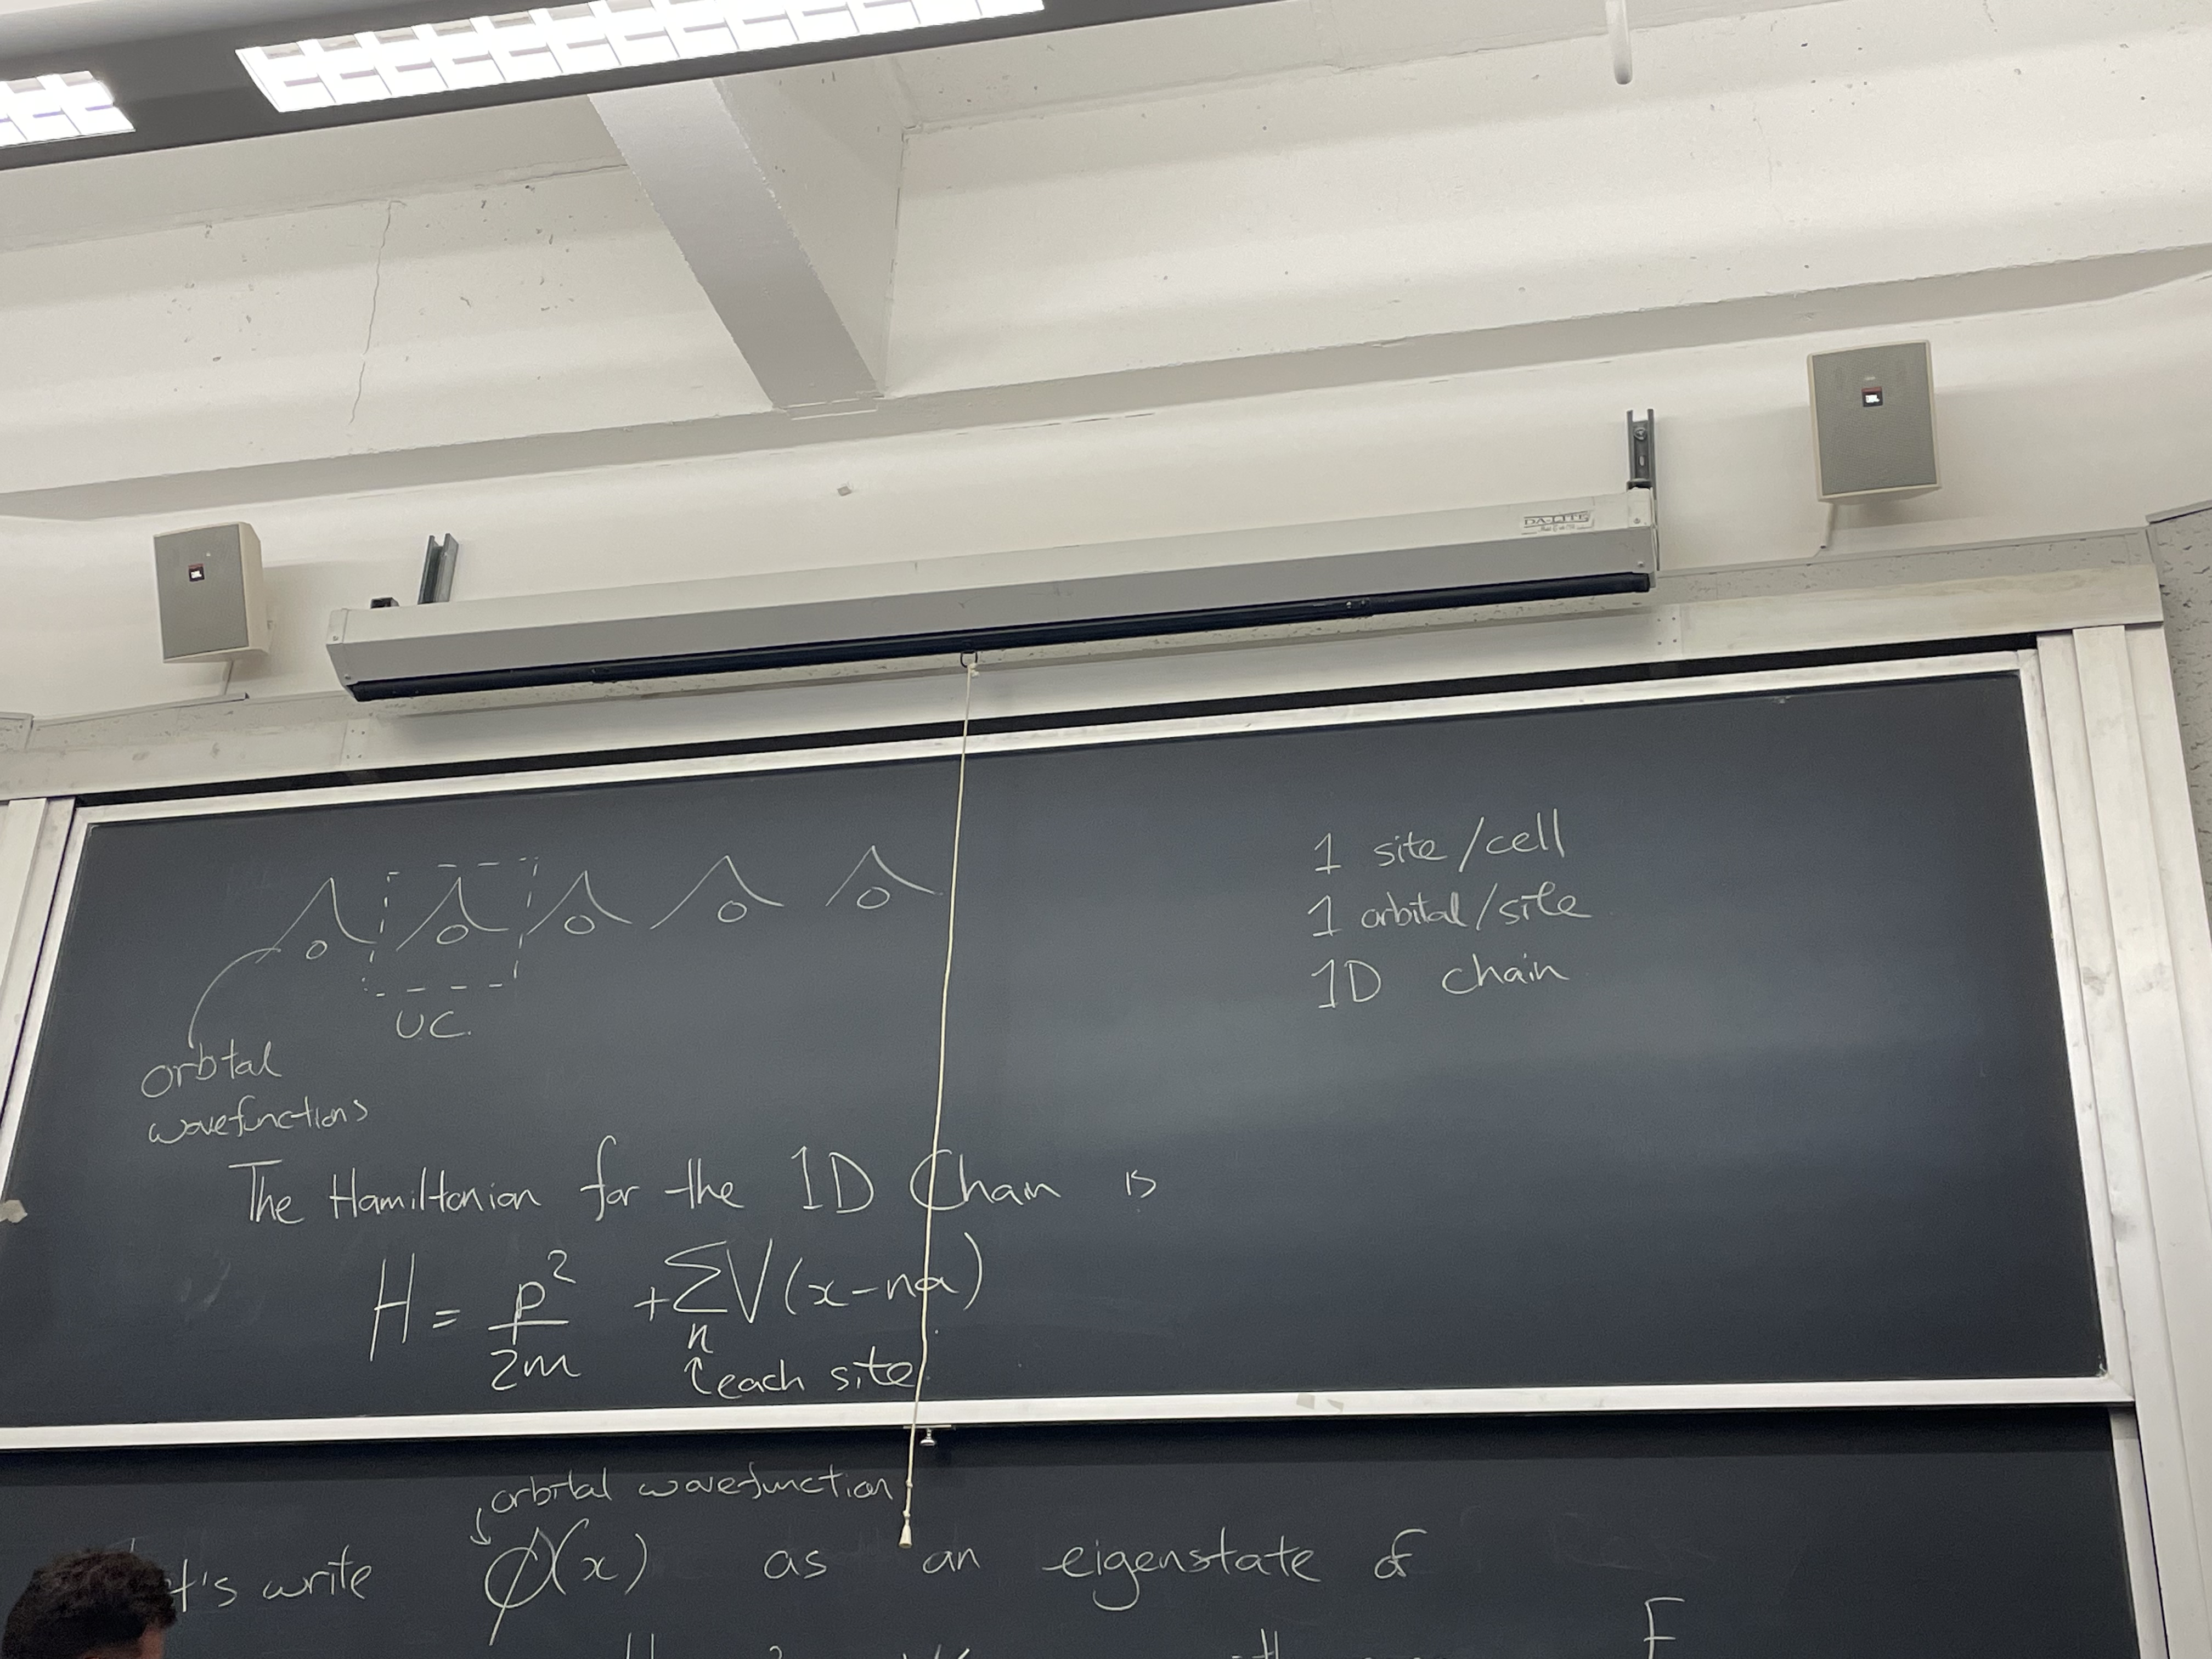
\includegraphics[scale=0.05]{Pictures/Jan 22/Tight-binding.png}
\end{center} The Hamiltonian for the 1D Chain is $$ H = \frac{\mathbf{p}^2}{2m} + \sum_{n} V(x-na) $$ Let $\phi(x)$ be the eigenstate of $$ H_0 = \frac{\mathbf{p}^2}{2m} + V(x) $$ with energy $E_0$ i.e. $\phi(x)$ is the \textbf{Orbital Wavefunction}. The Hilbert Space for the chain consists of one orbital at each site $\{\phi_n(x)\}_{n \in I}$ (the $n$ subscript labels the different sites) and the wavefunction for the chain is then $$ \boxed{\psi(x) = \sum_{n} c_n \phi_n(x - na)} $$ (linear combination of atomic orbitals) 

\vskip 1cm
\subsection{Review: Bloch's Theorem}
Next, we recall Bloch's theorem for a system with Translational Symmetry. Bloch's Theorem tells us that $$ \boxed{ \psi_k(x+a) = e^{ika} \psi_k(x) } $$ where $a$ is the size of the Unit Cell, which in this case is the distance between atoms \begin{note} {Add a proof} \end{note}.
\\
\\
From this, we can arrive at the conclusion that $$ c_n = c_0 e^{ikna} $$ and including the normalization, a chain of $N$ atoms is described by wavefunctions $$ \boxed{\psi_k(x) = \frac{1}{\sqrt{N}} \sum_{n} e^{ikna} \psi(x-na)  } $$ This can be interpreted as the single orbital wavefunction $\phi(x)$ being modulated by the free-electron wavefunction $e^{ikx}$.
\\
\\
The Energy Spectrum (or dispersion relation) is given by $$ E(k) = E_0 - 2t \cos(ka) $$ where $t$ is called the \textbf{Overlap integral} $$ t \equiv \int \mathrm{d}x ~ \phi(x) V(x) \phi(x-a) $$ \begin{center}
  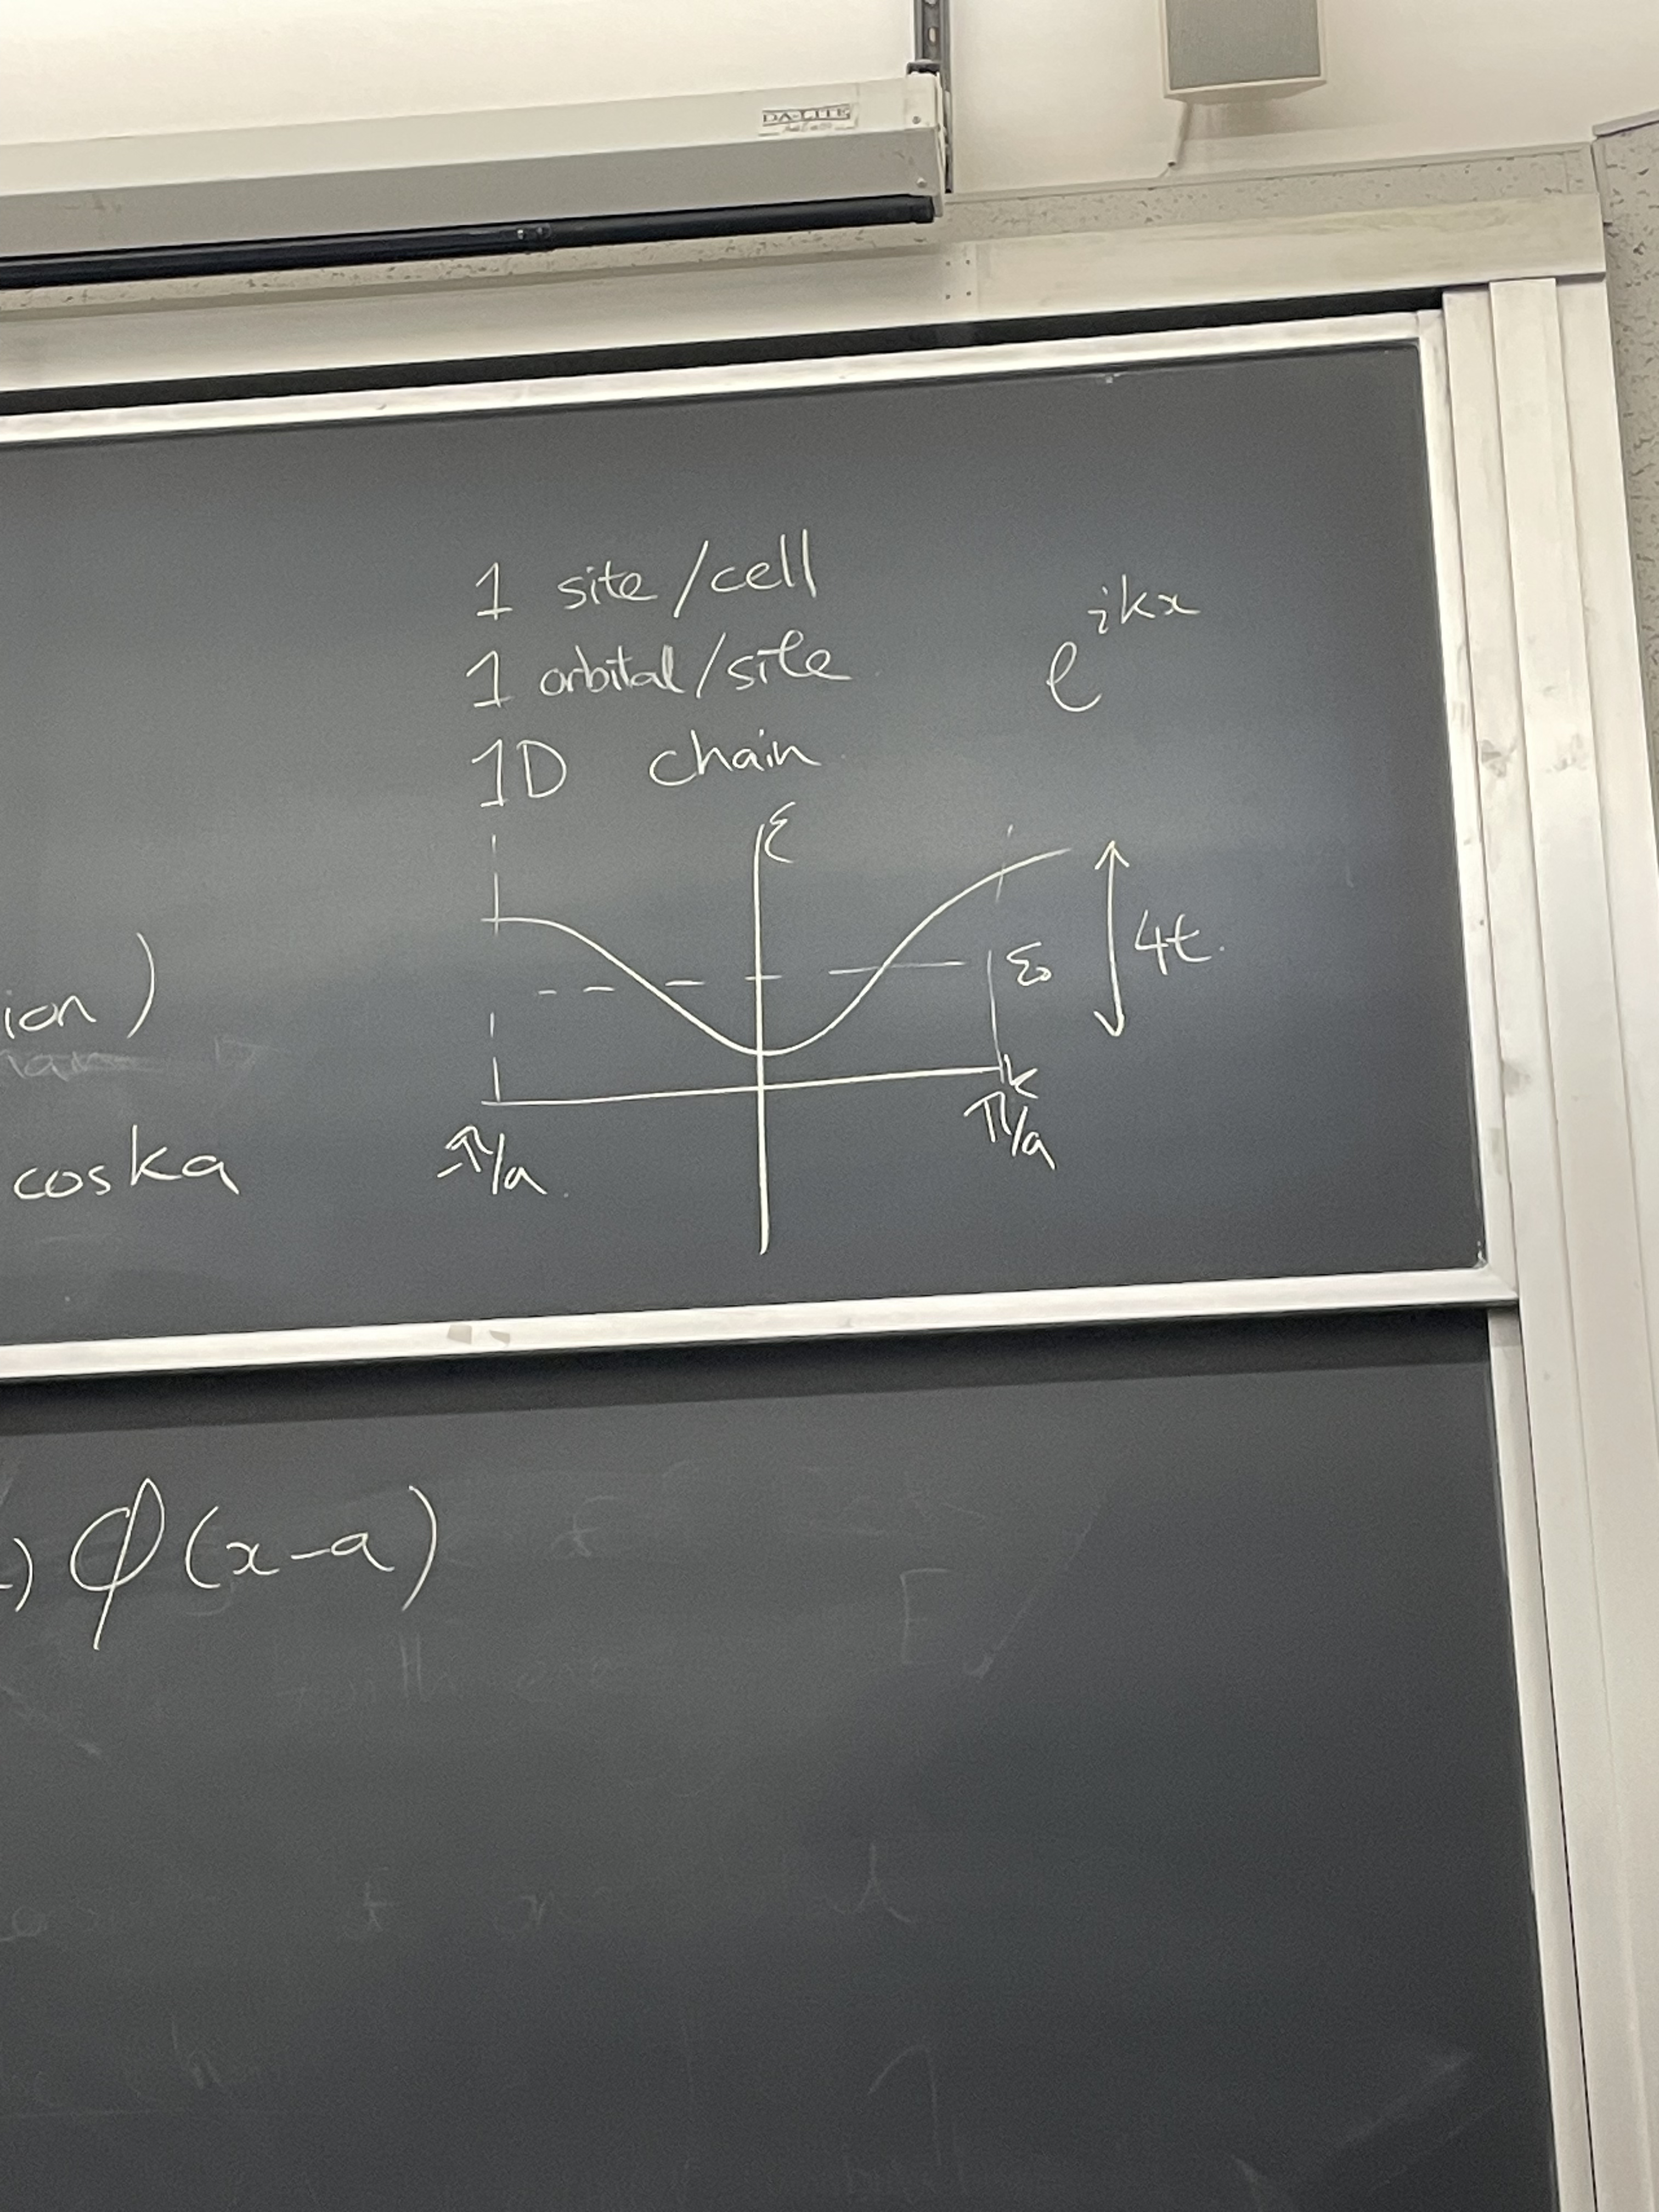
\includegraphics[scale=0.05]{Pictures/Jan 22/Tight-binding Dispersion.png}
\end{center} This model is too trivial to display any topological behavior. The physics we're interested in becomes apparent once we have \textbf{at least two bands \emph{and} a bandgap}. As our first case, we study the SSH model (Phys. Rev. Lett. 42 1698 (1979)).

\vskip 1cm
\subsection{SSH Model}
In the SSH model we, once again, have a 1D chain. However, this time, we have \textbf{two kinds of bonds} (alternating) with different overlap/hopping parameters $t_1, t_2$.
\begin{center}
  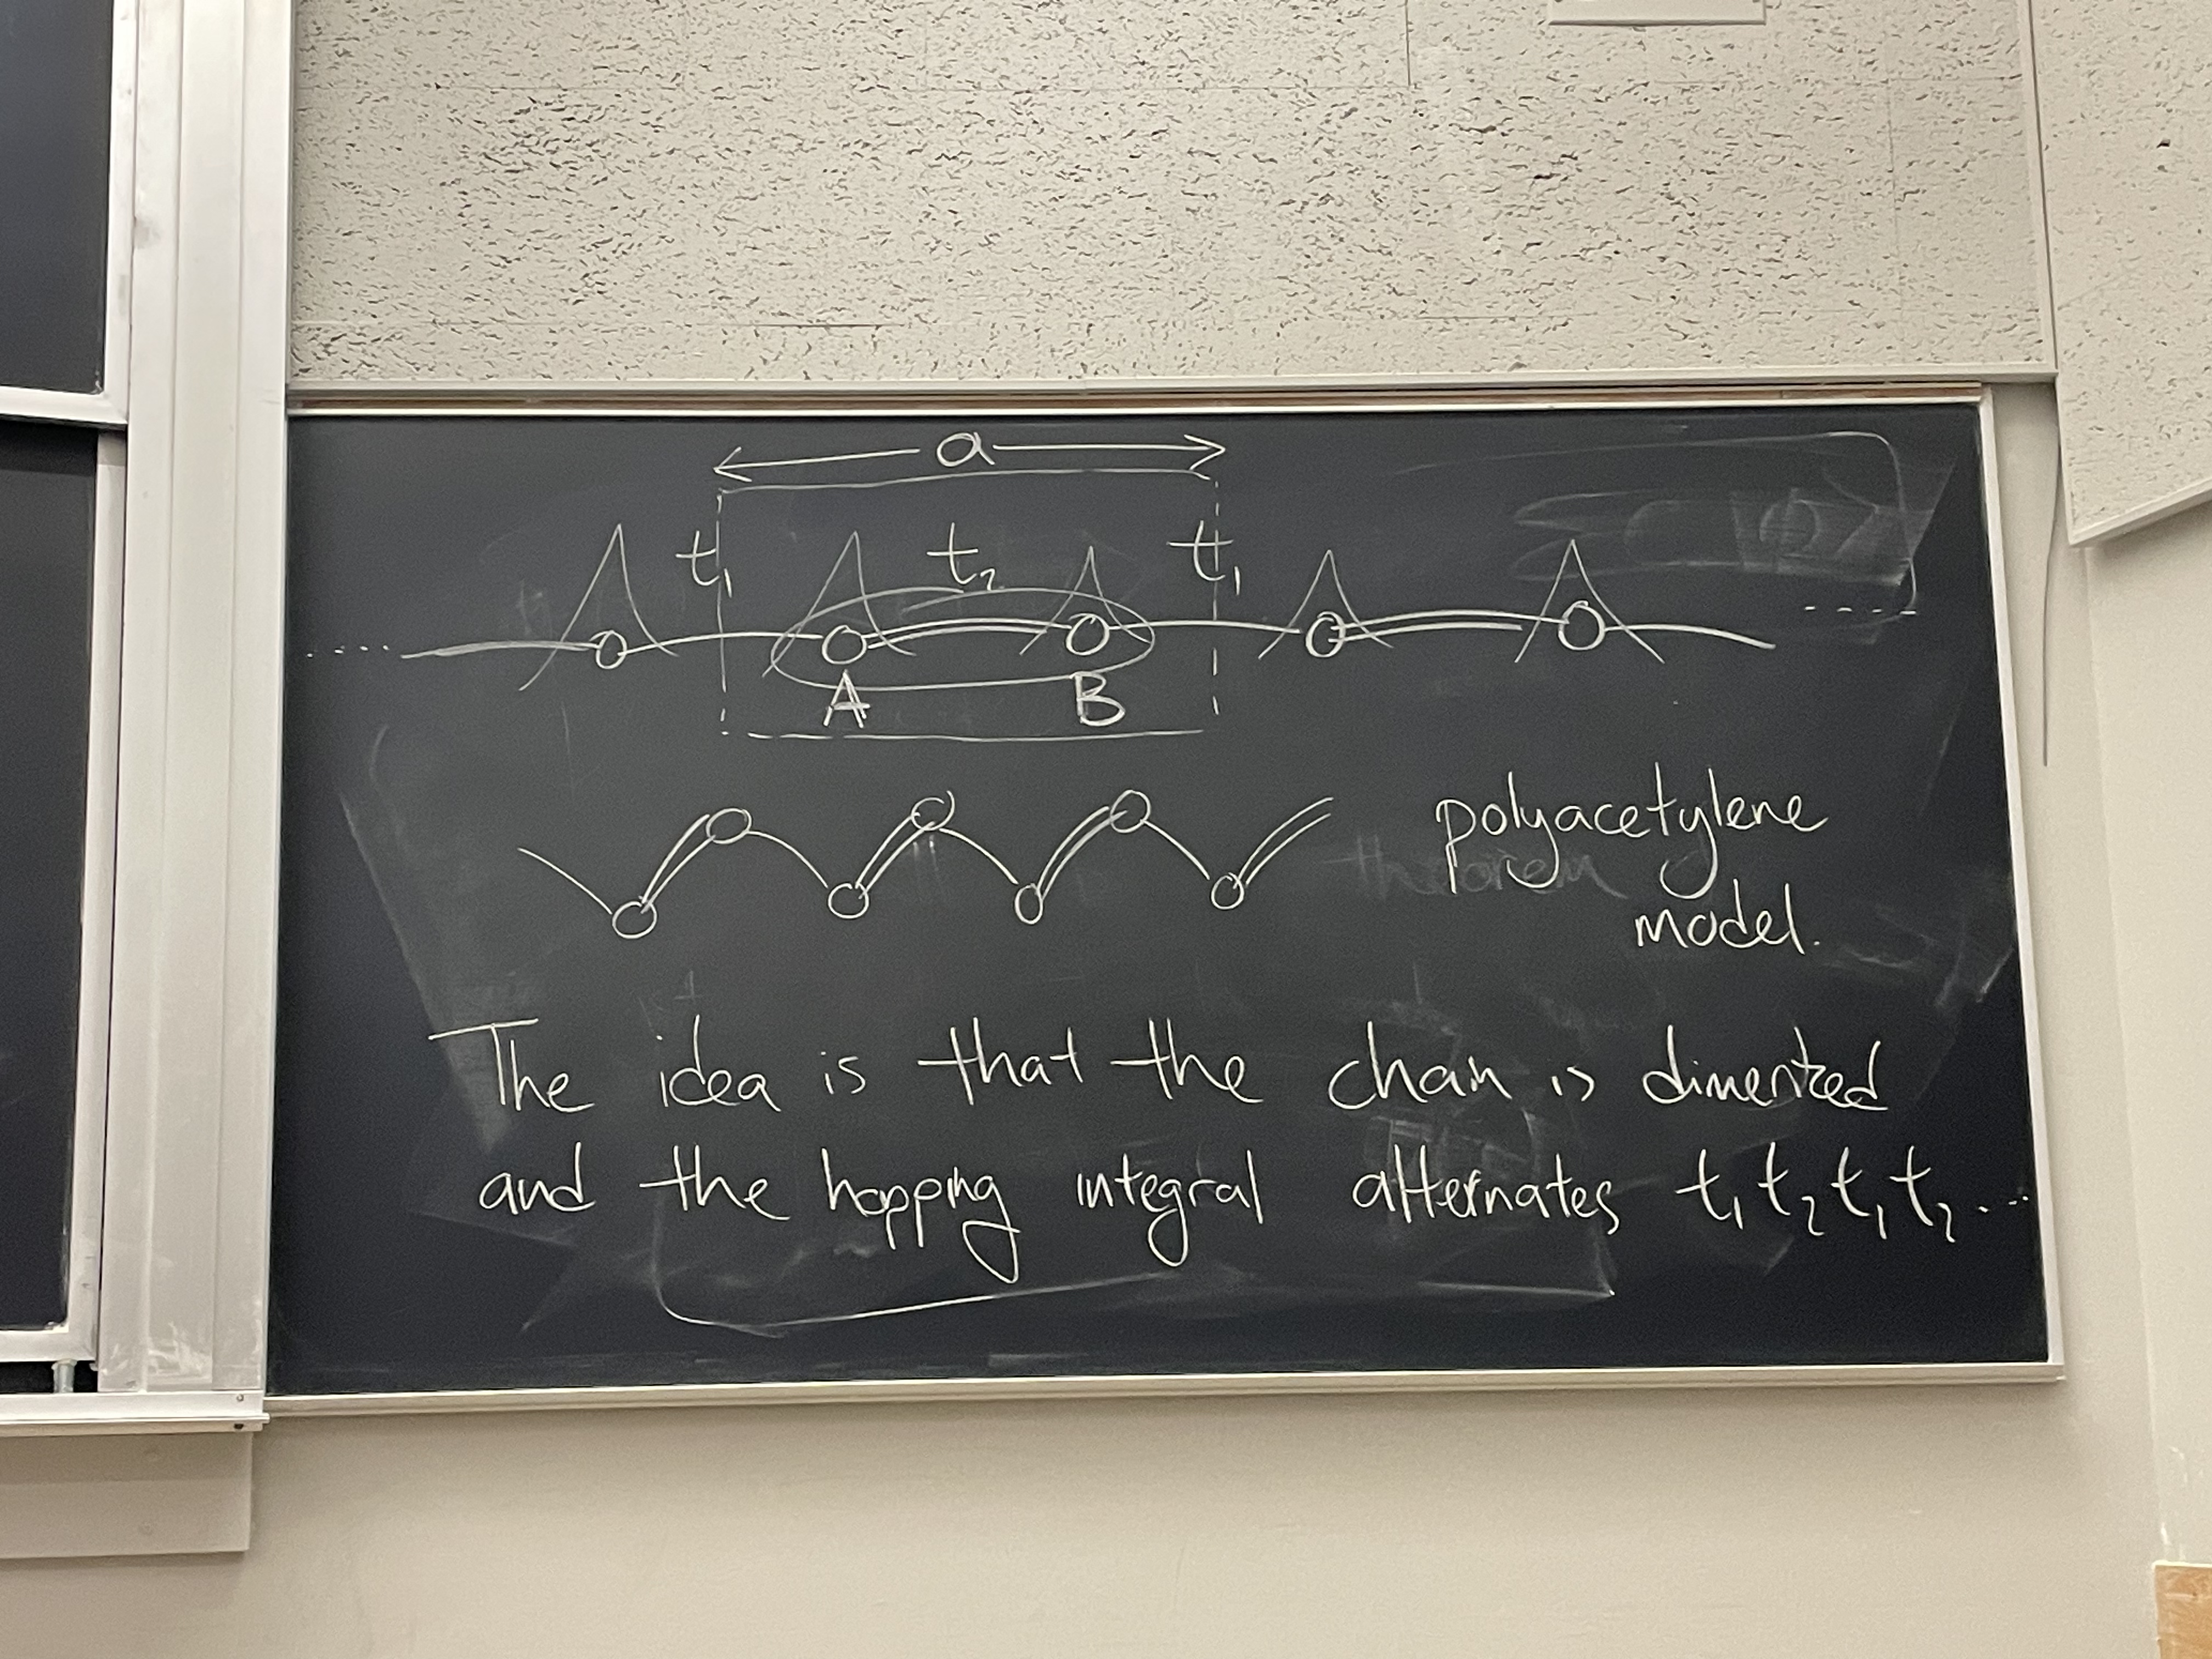
\includegraphics[scale=0.05]{Pictures/Jan 22/SSH Model.png}
\end{center}
For example, Polyacetylene is described by an SSH model. The idea is that the chain is \textbf{dimerised} because the hopping integral alternates.
\\
\\
The wavefunctions for this system are $$ \psi_k(x) = \frac{1}{\sqrt{N}} \sum_{n} e^{ikna} \left( \alpha_{k} \phi_{nA} + \beta_k \phi_{nB} \right) $$ where $a$ is the unit cell size and it is $2 \times$ the distance between sites. $\phi_{nA}, \phi_{nB}$ are the orbital waves on sites $A$ and $B$. 

\begin{redbox}
What are $\alpha_k, \beta_k$? \\
Probability amplitudes.
\end{redbox}

\begin{itemize}
  \item Now we need to solve the Schr\"odinger Equation to determine $\alpha_{k}$ and $\beta_k$. We know that $$ |\alpha_k|^2 + |\beta_k|^2  = 1 $$ 
  \item This is a 2D Hilbert Space
  \item We want to solve $H \psi_k(x) = E(k) \psi_k(x) $. To construct the matrix, take the product with $\bra{\phi_{nA}}$ and $\bra{\phi_{nB}}$, giving us the two equations 
  \begin{align*}
    \braket{\phi_{nA}}{H|\psi_k(x)} &= E(k) \braket{\phi_{nA}}{\psi_k} \\
    \braket{\phi_{nB}}{H|\psi_k(x)} &= E(k) \braket{\phi_{nB}}{\psi_k} \\
  \end{align*}

  \item Taking the first of these equations, the RHS is 
  \begin{align*}
    \braket{\phi_{nA}}{ \sum_{n'} e^{ikn'a} | \left( \alpha_k \phi_{n'A} + \beta_{k} \phi_{n'B} \right) }
  \end{align*} \begin{note}
    {missed a bit here}
  \end{note} So, the RHS is $E(k) \alpha_k e^{ikna} $

  \item Now, for the LHS, 
  \begin{align*}
    \sum_{n'} \braket{\phi_{nA}}{H|e^{ikn'a} \left(\alpha_{k} \phi_{n'A} + \beta_{k} \phi_{n' B}\right) } 
  \end{align*} 
  \item Recall that $H$ is described as $$ H = H_0 + \sum_{n'} V(x-n'a) $$ where $H_0 \ket{\phi_{n'A}} = E_0 $. When we take the inner product, only the $n=n'$ inner product survives when we dot with $H_0$, giving $$ \braket{\phi_{n'A}}{H_0|\left(\alpha_{k} \phi_{n'A} + \beta_{k} \phi_{n' B}\right)} = E_0 \alpha_k e^{ikna} $$
  \item The Second Term (only nearest neighbor hopping) is equal to 
  \begin{align*}
    &= e^{ikna} \braket{\phi_{nA}}{V_0(x-x_{n,B})| \beta_k \phi_{n,B} } + e^{ik(n-1)a} \braket{\phi_{nA}}{V_0(x-x_{n-1,B})| \beta_k \phi_{n-1,B} } \\
    &= \beta_k t_1 e^{ikna} + \beta_k t_2 e^{ik(n-1)a} \\
    &= \beta_k e^{ikna} \left( t_1 + t_2 e^{-ika} \right)
  \end{align*} 
\end{itemize}

\vskip 1cm
\hrule

%%%%%%%%%%%%%%%%%%%%%%%%%%%%%%%%%%%%%%%%%%%%%%%%
\pagebreak
\section{January 24, 2025:}
%%%%%%%%%%%%%%%%%%%%%%%%%%%%%%%%%%%%%%%%%%%%%%%%

Things get more interesting today. We won't reach the Topological aspects yet, but we'll cover them next Monday.
\\
\\
We left off looking at the LHS and RHS of the Schr\"odinger Equation for the SSH model, ending with the following equation: 
\begin{align*}
  &\alpha_k E_0 e^{ikna} + \beta_k t_1 e^{ikna} + \beta_k t_2 e^{ik(n-1)a} = \alpha_k E(k) e^{ikna} \\
  \implies& \alpha_k (E(k) - E_0) + \beta_k (t_1 + t_1 e^{-ika}) = 0 \\
\end{align*} Performing the same procedure, but taking the inner product with $\bra{\phi_{nB}}$ instead, we get a similar equation, giving us the following system of simultaneous equations:
\begin{align*}
  & \alpha_k (E(k) - E_0) + \beta_k (t_1 + t_1 e^{-ika}) = 0 \\ 
  & \beta_k (E(k) - E_0) + \alpha_k (t_1 + t_1 e^{+ika}) = 0 \\ 
\end{align*} For a 2D Hilbert Space (in this case, spanned by $\ket{\phi_{nA}}$ and $\ket{\phi_{nB}}$) we can regard the wavefunctions as "$S = 1/2$" \textbf{spinors} or "Pseudospins". 
\\
\\
Pseudospins or Spinors are objects of the form $$ \begin{pmatrix}
  \alpha_{k} \\ \beta_{k}
\end{pmatrix} $$ We can write these two simultaneous equations represented by this spinor as $$ \underbrace{\begin{pmatrix}
  E_0 & t_1 + t_2 e^{-ika} \\
  t_1 + t_2 e^{+ika} & E_0 \\
\end{pmatrix}}_{\text{"Bloch Hamiltonian"}} \begin{pmatrix}
  \alpha_k \\ \beta_k
\end{pmatrix} =  E(k) \begin{pmatrix}
  \alpha_k \\ \beta_k
\end{pmatrix} $$ where it's called the "Bloch Hamiltonian" because everything is represented in $k$-space. The Bloch Hamiltonian has the form $$ H(k) \underbrace{\vec{\phi}_k}_{\text{Spinor}} = E(k) \vec{\phi}_k $$ Generally, a Bloch Hamiltonian is an $N \times N$ matrix where $$ N = \begin{pmatrix}
  \text{\# sites} \\
  \text{per U.C.} \\
\end{pmatrix} \times \begin{pmatrix}
  \text{\# orbitals} \\
  \text{per site} \\
\end{pmatrix} \times \begin{pmatrix}
  \text{\# of} \\
  \text{dimensions} \\
\end{pmatrix}  $$ So, in our case, we have $N = 2 \times 1 \times 1 = 2$ We solve our $2 \times 2$ matrix in the usual way. 

\vskip 1cm
\subsection{What is the "Pseudospin" representation?}
The Pseudospin is the $2$-state system of each allowed value of momentum $k$.

\vskip 1cm
\subsubsection*{But what do $\alpha_k$ and $\beta_k$ represent?} 
\vskip 0.5cm
\begin{center}
  Include figure of B and A sublattices (blue and yellow)
\end{center} We visualize these as two interpenetrating sublattices. Basically, $\alpha$ and $\beta$ refer to the wavefunctions on the $A$ and $B$ sublattices respectively, but let's take this idea a little further.
\\
\\
Any $2 \times 2$ matrix can be represented as a linear superposition of Pauli matrices and the identity. 
\begin{align*}
  \text{Pauli Matrices:} ~ \sigma_x = \begin{pmatrix}
    0 & 1 \\
    1 & 0
  \end{pmatrix}, ~ \sigma_y = \begin{pmatrix}
    0 & -i \\
    i & 0
  \end{pmatrix}  ~ \sigma_z = \begin{pmatrix}
    1 & 0 \\
    0 & -1
  \end{pmatrix},  ~ \sigma_0 = \mathbf{1} = \begin{pmatrix}
    1 & 0 \\
    0 & 1
  \end{pmatrix}
\end{align*} Let us represent our Bloch Hamiltonian as 
\begin{align*}
  H(k) = \begin{pmatrix}
    E_0 & \Delta(k) \\
    \Delta^*(k) & E_0 \\
  \end{pmatrix}, ~ \Delta(k) = t_1 + t_2 e^{-ika}
\end{align*} Then, solving the Schr\"odinger Equation amounts to solving 
\begin{align*}
  &\mathrm{det} \begin{bmatrix}
    E_0 - E(k) & \Delta(k) \\
    \Delta^*(k) & E_0 - E(l)
  \end{bmatrix} = 0 \\
  \implies& E_0 - E(k) = \pm \left| \Delta(k) \right| \\
  \implies& \left| \Delta(k) \right| = \left| t_1 + t_2 e^{ika} \right| = \sqrt{t_1^2 + t_2^2 + 2t_1t_2 \cos(ka)}
\end{align*} 

\subsubsection*{The Band Structure}
For the sake of convenience let's set $E_0 = 0$. Now, we have 
\begin{align*}
  &k = 0 \implies \Delta(0) = |t_1 + t_2| \\
  &k = \frac{\pi}{a} \implies \Delta(\frac{\pi}{a}) = |t_1 - t_2| 
\end{align*}
\begin{center}
  Include figure of the Band Structure.
\end{center} Notice that the band structure just depends on $|t_1 - t_2|$ and so doesn't actually care which one is bigger. \begin{note}
  {Ask for clarification}
\end{note} \\
\\
Now that we have the Band Structure, let's get back to the psuedospin wavefunctions 
\begin{align*}
  &\Delta(k) = \underbrace{\Delta_1(k)}_{\mathrm{Re}(\Delta(k))} +  \underbrace{i\Delta_2(k)}_{\mathrm{Im}(\Delta(k))}
\end{align*} So 
\begin{align*}
  H(k) &= \begin{pmatrix}
    E_0 & \Delta_1 + i \Delta_2 \\
    \Delta_1 - i \Delta_2 & E_0 \\
  \end{pmatrix} = E_0 \begin{pmatrix}
    1 & 0 \\
    0 & 1
  \end{pmatrix} + \Delta_1 \begin{pmatrix}
    0 & 1 \\
    1 & 0
  \end{pmatrix} + \Delta_2 \begin{pmatrix}
    0 & i \\
    -i & 0
  \end{pmatrix} \\
  &= E_0 \mathbf{1} + \Delta_1 \sigma_x - \Delta_2 \sigma_{y} + 0 \sigma_z
\end{align*} Now, since we have $E_0 = 0$ we can write 
\begin{align*}
  H(k) &= \vec{\sigma} \cdot \vec{b}(k)
\end{align*}
where \begin{align*}
  &\vec{b}_x = \begin{pmatrix}
    \Delta_1(k) \\ 0 \\ 0
  \end{pmatrix}, ~\vec{b}_y = \begin{pmatrix}
    0 \\ \Delta_2(k) \\ 0
  \end{pmatrix}, ~\vec{b}_z = \begin{pmatrix}
    0\\ 0 \\ 0
  \end{pmatrix} \\
  \text{ and }& \vec{b}(k) = b_x \hat{x} + b_y \hat{y} + b_z \hat{z}
\end{align*} This looks a lot like a spin in a magnetic field, and so we identify $\vec{\sigma}$ as being our pseudospin or spinor and $\vec{b}(k)$ as being our "Zeeman" field.
\\
\\
Note that there is no $\vec{\sigma}_z$ component. This follows from the fact that  the orbitals on site $A$ and $B$ are the same, and we have only allowed nearest neighbor hopping. If we did not restrict to nearest neighbors, we'd need to have a third parameter, but we would also lose all topological properties of the model (we'll show this later).
\\
\\
Now, in our case, the Hamiltonian only consists of $\sigma_x, \sigma_y$ and we know the Pauli matrices anti-commute with each other. As a result, $\sigma_z$ anticommutes with the Hamiltonian $\{\sigma_z, H\} = 0 $.
\\
\\
This is actually a special case of when some unitary operator $\Theta$ actos on $H$ as $$ \Theta H \Theta^{\dagger} = -H $$ The existence of such a relationship implies for $H \ket{\psi} = E\ket{\psi}$. that there exists another eigenstate with energy $-E$.  
\\
\\
This is a kind of \textbf{Chiral} symmetry, and such symmetries have very special consequences for the eigenvalues and are intimately related to the Topology in such systems.
\\
\\
We'll see later how this is a chiral symmetry in the sense of breaking all mirror symmetries.

\vskip 1cm
\hrule

%%%%%%%%%%%%%%%%%%%%%%%%%%%%%%%%%%%%%%%%%%%%%%%%
\pagebreak
\section{January 27, 2025:}
%%%%%%%%%%%%%%%%%%%%%%%%%%%%%%%%%%%%%%%%%%%%%%%%

Last time, we left off by expressing the SSH Hamiltonian in the form $$ H = \alpha \vec{\sigma} \cdot \vec{b} $$ where $\vec{b}(k) = (t_1 + t_2 \cos(ka))\hat{x} + t_2 \sin(ka) \hat{y}$. 

\begin{itemize}
  \item The point of $\vec{b}(k)$ helps us visualize the spinor wavefunctions, and the topological aspects of the SSH model will become apparent through the visualization.
  
  \item For each wavenumber $k$, the two eigenstates are "Pseudospin" states that are parallel and anti-parallel to the "Spinor field" $\vec{b}(k)$. These are separated in energy by $2|\vec{b}(k)|$.

  \item This is where things get a bit more geometrical... We can trace the trajectory of $\vec{b}(k)$ as $k$ varies across the 1D Brillouin zone from $-\pi/a$ to $\pi/a$.
  
  \item In general, for 1D, this is a map from a circle (obtained by connecting the ends of the 1D BZ) to a surface in 3D (since $\vec{b}(k)$ has three components).
\end{itemize}

\begin{center}
  Include figure
\end{center}

\begin{itemize}
  \item For the SSH model with chiral symmetry (as discussed last lecture), $b_z(k) = 0$ (no $\hat{z}$ component) of $\breve{b}(k)$.
  
  \item So, $\vec{b}(k)$ vectors actually lie on the $xy$-plane and the surface becomes a contour in the $xy$-plane.
\end{itemize}

\begin{center}
  Include figure
\end{center} Let's calculate some important values of $\vec{b}(k)$ as we move across the BZ from $-\pi/a$ to $\pi/a$ and we'll consider $t_1 > t_2$
\begin{itemize}
  \item $\vec{b}(-\pi/a) = (t_1 - t_2)\hat{x} + 0\hat{y}$
  \item $\vec{b}(-\pi/2a) = t_1\hat{x} -t_2 \hat{y}$
  \item $\vec{b}(0) = (t_1 + t_1)\hat{x} + 0\hat{y}$
  \item $\vec{b}(\pi/2a) = t_1\hat{x} + t_2 \hat{y}$
  \item $\vec{b}(\pi/a) = (t_1 - t_2)\hat{x} + 0\hat{y}$
\end{itemize}

\begin{center}
  Include figure
\end{center}

\begin{itemize}
  \item The interesting bit is that this conclusion for the trajectory of $\vec{b}(k)$ depends on the relative magnitudes of $t_1$ and $t_2$.
  
  \item Above, we assumed $t_1 > t_2$. What about the opposite case where $t_2 > t_1$? We might imagine that our solutions would be exactly the same since 
  \begin{itemize}
    \item energy states are the same (bandstructure only depended on $|t_1 - t_2|$), and
    \item the physical situation looks the same.
  \end{itemize}
\end{itemize}

\begin{center}
  Include figure
\end{center} 

\begin{itemize}
  \item However, when we look at the trajectory of $\vec{b}(k)$ in the $t_2 > t_1$ case, it's actually \color{blue} different \color{black} than the $t_1 > t_2$ case.
  
  \item More precisely, they are \textbf{Topologically Distinct} (we'll elaborate on what this means).
\end{itemize} The expressions remain the same, \begin{itemize}
  \item $\vec{b}(-\pi/a) = (t_1 - t_2)\hat{x} + 0\hat{y}$
  \item $\vec{b}(-\pi/2a) = t_1\hat{x} -t_2 \hat{y}$
  \item $\vec{b}(0) = (t_1 + t_1)\hat{x} + 0\hat{y}$
  \item $\vec{b}(\pi/2a) = t_1\hat{x} + t_2 \hat{y}$
  \item $\vec{b}(\pi/a) = (t_1 - t_2)\hat{x} + 0\hat{y}$
\end{itemize} it's just that we now have $t_2 > t_1$. But because of this, the first point is to the \textbf{left of the origin}. The rest of the points are also correspondingly offset, so the contour looks like the same circle but shifted over.

\begin{center}
  Include figure
\end{center}

\begin{itemize}
  \item $t_1 > t_2$: $\vec{b}(k)$ \underline{only} points East. 
  \item $t_2 > t_1$: $\vec{b}(k)$ points in all directions (N, S, E, W, etc.) and the trajectory encloses the origin.
  \item Sometimes it's easier to visualize using unit vectors $$ \hat{b}(k) = \frac{\vec{b}(k)}{|\vec{b}(k)|} $$ In this case, $\hat{b}(k)$ for $t_1 > t_2$ only traces out an arc on the Unit sphere wherease for $t_2 > t_1$ it traces out the full circle.
\end{itemize}

\begin{center}
  Include two figures
\end{center} These two states correspond to different \textbf{Solid Angles} $\Omega = 0$ for $t_1 > t_2$ and $\Omega = 2\pi$ for $t_2 > t_1$. The solid angle is directly proportional to the \textbf{Berry Phase} (we'll derive this result later) which is itself related to the \textbf{Chern Number} - a topological invariant. Thus, the $\Omega = 0$ case is Topologically Trivial, whereas the $\Omega = 2\pi$ case is \textbf{topologically non-trivial}. 
\\
\\
Now, there is some critical point between the $t_1 > t_2$ and $t_2 > t_1$ cases where the circle just touches the origin.
\begin{center}
  Include figure
\end{center} We define a "winding number" $W$ which is $0$ or $1$ and measures how many times the mapping encloses the Origin i.e. how many times $\vec{b}(k)$ covers the entire circle.

\begin{itemize}
  \item In order to go from $W = 0$ to $W = 1$, we must go through the origin. This means $\vec{b}(k) = 0$ for some $k$. 
  \item Recall that the energy gap between the negative and positive eigenstates was $2|\vec{b}(k)|$. 
  \item This means that in order to go from $W = 0$ to $W = 1$, we must close the energy gap!
  \item So, in order to Adiabatically go through the topological transition from $W = 0$ to $W = 1$ we must close the gap and there are zero-energy states.
\end{itemize}

\begin{redbox}
  This is an important property of topological systems! In order to go between topologically distinct states, the energy gap must close.
\end{redbox}

\begin{bluebox}
  What do we mean by \textbf{Adiabatic}?
  \\
  \\
  Roughly, we mean changing things slowly enough that none of the quantum numbers for the system change. See the \textbf{Adiabatic Theorem}.
\end{bluebox} Next time, we'll see what happens to the Winding number exactly when the energy gap closes and how that relates to Edge States.

\vskip 1cm
\hrule


%%%%%%%%%%%%%%%%%%%%%%%%%%%%%%%%%%%%%%%%%%%%%%%%
\pagebreak
\section{January 29, 2025:}
%%%%%%%%%%%%%%%%%%%%%%%%%%%%%%%%%%%%%%%%%%%%%%%%

\begin{itemize}
  \item Last time, we left off discussing Winding Numbers, which characterized the cases $t_1 > t_2$ and $t_2 > t_1$, making them distinct topological phases.
  
  \item Note that in general 1D systems, we don't have distinct topological phases. The SSH model is special because of the restriction that the Hamiltonian only contains $\sigma_x$ and $\sigma_y$.
  
  \item If we allow the $\sigma_z$ term to be finite so that the Hamiltonian is of the form $$ H = \beta_x(k) \sigma_x + \beta_y(k) \sigma_y + \beta_z(k) \sigma_z $$ we cannot generally define a winding number.
  
  \item The reason has to do with the bandgap. For the SSH model, in order to go from the $W=0$ to $W=1$ case, we need to close the bandgap. However, if the $\sigma_z$ term is non-zero, we can transform between them adiabatically without needing to close the gap because we allow $b_z$ to help us evolve continuously. \begin{note}
    {Find more detailed discussion in Asboth 1.5}
  \end{note}
\end{itemize}

\begin{center}
  Include figure
\end{center} WE need to go to higher dimensions to see examples of "generic" insulating states with topological invariants that cannot be changed without closing a gap.

\vskip 1cm
\subsection{Are there observable consequences?}

\begin{itemize}
  \item In the bulk, there's no physical difference. 
  \item The relevant observables are seen at the boundaries between the two situations i.e. the $W = 0$ chain and the $W = 1$ chain.
  \item To see this, we consider the fully dimerised limit (meaning make $t_1$ finite and make $t_2 = 0$ or vice-versa), whose solutions are essentially the same for a bunch of diatomic molecules.
\end{itemize}

\begin{center}
  Include Figure
\end{center}

\begin{itemize}
  \item Consider the boundaries of a finite chain. \begin{thought}
    {An infinite chain is not useful to us because in that case, the $W = 0$ and $W = 1$ cases only differ by a translation of $a$ and cannot be different.}
  \end{thought}

  \item Imagine the system is $1/2$ filled. 
\end{itemize}

\begin{center}
  Include figure of the dispersion for 1/2 filled
\end{center} There is one electron per dimer.

\begin{itemize}
  \item  In the first situation, the electron sits happily on each dimer. \begin{center}
    Include fig
  \end{center}
  \item In the second situation, we have just as many sites and therefore just as many electrons, but now one electron sits at a single site rather than being shared. As a result, one site has $+\frac{1}{2}e$ more than expected from the bulk and the other has $-\frac{1}{2}e$ less than expected. \begin{center}
    Include figure
  \end{center}

  \item The boundary states in each situation look different! The topological system $W=1$ has $\pm \frac{1}{2} e$ more (less) than expected at its ends!
\end{itemize}

\subsection*{What happens if we have an odd number of sites instead?} We can make a similar argument, but we'd have to tile the system differently. \begin{note}
  {Exercise: Analyse the SSH model with 7 sites.}
\end{note}

\vskip 1cm
\subsection*{Band Structure for Fully Dimersized System}

\begin{center}
  Include fig
\end{center}

\subsection{Boundary states from another perspective}

\begin{itemize}
  \item Consider a domain wall between a $W = 0$ and $W = 1$ system. \begin{center}
    Include fig
  \end{center} 
  \item At the boundary, there is a non-bonded atom at energy $E_0$ (the atomic energy) or $E - E-0 = 0$.
  \item This is a zero energy state! So, in order to cross between topolgically distinct states, we have to close the gap (move through the zero energy state). This is consistent with the idea that the gap must close in order to go from one topological phase to another.
\end{itemize}

\vskip 1cm
\subsection*{What happens if we relax the dimerization condition?} The boundary state remains pinned to $E - E_0 = 0$ and gap remains in order for the system to maintain its Chiral Symmetry.
\\
\\
Next time, Berry Phases in Higher Dimensional Systems.


%%%%%%%%%%%%%%%%%%%%%%%%%%%%%%%%%%%%%%%%%%%%%%%%
\pagebreak
\section{Janary 31, 2025:}
%%%%%%%%%%%%%%%%%%%%%%%%%%%%%%%%%%%%%%%%%%%%%%%%

Missed lecture. Fill in later.

%%%%%%%%%%%%%%%%%%%%%%%%%%%%%%%%%%%%%%%%%%%%%%%%
\pagebreak
\section{February 3, 2025:}
%%%%%%%%%%%%%%%%%%%%%%%%%%%%%%%%%%%%%%%%%%%%%%%%

Picking up where we left off last time, we'll move from the finite to continuous case of the Berry phase.
\\
\\
Recall that we considered the following triangle lattice situation, 
\begin{center}
  Include figure
\end{center} with a tight-binding Hamiltonian $$ H = \begin{pmatrix}
  0 & -t & -t \\
  -t & 0 & -t \\
  -t & -t & 0 \\
\end{pmatrix} $$ We Diagonalized it and found the energies and corresponding eigenstates.
\begin{center}
  Include figure of energy
\end{center} 
\begin{itemize}
  \item Eigenvectors have to be complex for the Berry's Phase to make any sense \begin{note}{write why exactly this is the case}\end{note}.
  \item In our case, the "loop" corresponds to rotations of a "distorted triangle".
\end{itemize}
\begin{center}
  Include fig of distorted triangle being rotated and corresponding hamiltonians
\end{center} 
\begin{itemize}
  \item Recall that the entries of the tight-binding hamiltonian are exactly the hopping parameters between the different lattice sites (since we're taking $E_0 = 0$) and so we just need to modify the hopping parameters in whatever row corresponds to the double-bond.
  
  \item The original equilateral triangle has two degenerate states $\ket{\alpha}$ and $\ket{\beta}$ that we will now use as a basis to describe a distored triangles energy levels.
  
  \item Consider the lower of the two degenerate undistorted energies after they are split by the distortion. Call this state $\ket{u_{i}}$ where $i \in \{a,b,c\}$
\end{itemize}

\begin{center}
  Include figure of energy splitting.
\end{center} Now we're going to do something that might seem a bit ad-hoc. We're going to assume that the following expressions hold true: 

% \begin{align*}
%   \ket{u_a} &= \frac{1}{\sqrt{2}} \left( \ket{\alpha} +  \ket{\beta} \right) = \frac{1}{\sqrt{2}} \begin\begin{pmatrix}
%     1 \\ 1
%   \end{pmatrix} \\
%   \ket{u_b} &= \frac{1}{\sqrt{2}} \begin{pmatrix}
%     1 \\ e^{i2\pi/3}
%   \end{pmatrix} 
% \end{align*} 
\begin{note}
  {Fill in the expressions above from picture}
\end{note}
\\
\\
Now, the expression for the Berry Phase we'll use is 
$$ \phi = - \mathrm{Im} \left( \mathrm{ln} \braket{u_a}{u_b} \braket{u_b}{u_c} \braket{u_c}{u_a} \right) $$ where the negative sign is just there by convention \begin{note}
{Read about why this is up to convention}
\end{note} 
\\
\\
Anyway, this comes out to 
\begin{align*}
  \phi &= -\mathrm{Im} \left( \mathrm{ln} \left(e^{i\pi/3}\right)^3 \right) \\
  &= -\pi
\end{align*} (It's important to use a complex space, otherwise you will have only $\phi = 0$ or $\phi = \pi$ for purely real eigenvectors).

\begin{itemize}
  \item The point of this is that if I multiply by a phase this product ($\phi$) will be invariant i.e. if we multiplied each eigenvector by a (possibly different) phase $$ \ket{\tilde{u_j}} = e^{i\beta_j} \ket{u_j} $$ it would not affect $\phi$ because the inner product comes with partnets of bras and kets $\ket{u_j}\bra{u_j}$ and so the extra phases cancel $$ e^{-i\beta_j} e^{i\beta_j} $$
  
  \item Also recall that $\mathrm{ln}(AB) = \mathrm{ln}(A) + \mathrm{ln}(B)$ so 
\end{itemize}

\begin{align*}
  \phi &= -\sum_{j = 0}^{N-1} \mathrm{Im} \left( \mathrm{ln}\left( \braket{u_j}{u_{j+1}} \right)\right)
\end{align*}

 \begin{itemize}
  \item But there's some subtely here. In our first definition for $\phi$, we have the restriction $\phi \in [-\pi, \pi]$
  \item But in this summation expression, we only have equivalence between $\phi$ values up to a phase of $2\pi$.
  \item So, we make sure that we define $\phi$ modulo $2\pi$ - this becomes important for equalities in our calculations.
\end{itemize} 

\vskip 1cm
\subsection{Parallel Transport Gauge}
Since we are free to choose a gauge (choice of phase to multiply the wavefunctions by), we can define each consecutive eigenstate along our loop as having the phase $$ \ket{\bar{u}_0} = \ket{u_0} $$ but then define $\ket{\bar{u}_1}$ such that $\braket{\bar{u}_0}{\bar{u}_1}$ is real.
\begin{center}
  Include figure of loop with kets and bar'd kets
\end{center} In this gauge, we have $$ \mathrm{Im} \left(\braket{u_j}{u_{j+1}}\right) = 0 $$ and the eigenvectors are "parallel" in the sense taht their relative phase is zero.
\begin{center}
  Include figure of "parallel"
\end{center}

\begin{itemize}
  \item However there is an awkwardness about the gauge.
  \item Before, we had $ \ket{u_0} \equiv \ket{u_N} $ but now, $\ket{\bar{u}_0} \not\equiv \ket{\bar{u}_N}$. They now differ by a phase - in fact, they differ exactly by  a Berry;s phase.
\end{itemize}

\vskip 1cm
\subsection*{An example computation}
Consider $ \ket{\bar{u}_a} = \ket{u_a} = \begin{pmatrix}
  1 \\ 1
\end{pmatrix} $ and now we need to define $\ket{\bar{u}_b}$ in terms of $\ket{u_b} = \begin{pmatrix}
1 \\ e^{i2\pi/3}
\end{pmatrix}$ so that $\mathrm{Im}\braket{\bar{u}_a}{\bar{u}_b} = 0$ 
\\
\\
Let's define $\ket{\bar{u}_b} = \begin{pmatrix}
  \alpha \\ \beta
\end{pmatrix}$. Then, $\braket{\bar{u}_a}{\bar{u}_b} = \alpha + \beta = \text{ Real }$ So, then, let's define $\ket{\bar{u}_b} = e^{-i\pi/3} \ket{u_b}$ giving us $$ \braket{\bar{u}_a}{\bar{u}_b} = e^{-i\pi/2} + e^{i\pi/3} = 2\cos\pi/3 = -1$$
\\
\\
repeating the procedure we get \begin{note}
  {Fill in from picture}
\end{note} 
\\
\\
But now there is a discontinuity in the phase as we move along the closed path. This is what people sometimes refer to when they say we need to "unwind" the phase by $\pi$ to go from $\ket{\bar{u}_N}$ to $\ket{\bar{u}_0}$. To avoid this awkward discontinuity we can instead use the Twisted Parallel Transport Gauge.

\vskip 1cm
\subsection{Twisted Parallel Transport Gauge}
In this gauge, we define $$ \ket{\tilde{u}_j} = e^{-i(\phi/N)j} \ket{\bar{u}_j} $$ This is a way of "continuously unwinding" the Berry Phase.


%%%%%%%%%%%%%%%%%%%%%%%%%%%%%%%%%%%%%%%%%%%%%%%%
\pagebreak
\section{February 5, 2025:}
%%%%%%%%%%%%%%%%%%%%%%%%%%%%%%%%%%%%%%%%%%%%%%%%

Last time, we left off discussing the Twisted Parallel transport Gauge. The idea is that the phase evolves by the same amount at each step as we parallel transport.

\subsection*{Twisted Parallel Transport Gauge continued...}

In this gauge, we define $$ \ket{\tilde{u}_j} = e^{-i(\phi/N) j} \ket{\bar{u}_j} $$ where $\ket{\bar{u}_j}$ is an eigenstate in the Parallel Transport Gauge and there is no discontinuity between $\ket{\tilde{u}_0}$ and $\ket{\tilde{u}_N}$, like there is in parallel transport gauge.

\vskip 1cm
\subsection{Continuous Formulation of the Berry Connection}
\begin{thought}
  {We're following David Vanderbilt's "Berry Phases in Electronic Structure Theory CHS" for this section.}
\end{thought} This time instead of having discrete steps, we take our path to be parameterized by a continuous variable $\lambda$ such that $\ket{u_{\lambda}}$ traverses a closed path going from $\lambda = 0$ to $\lambda = 1$ i.e. $$ \ket{u_{\lambda = 0}} \equiv \ket{ u_{\lambda = 1}}  $$ We assume that $\ket{u_{\lambda}}$ is a continuously differentialbe function of $\lambda$.
\\
\\
Now,
\begin{align*}
  \mathrm{ln}\left(\braket{u_{\lambda}}{u_{\lambda+d\lambda}}\right) &= \mathrm{ln} \left( \braket{u_{\lambda}}{u_{\lambda}} + d\lambda \braket{u_{\lambda}}{\frac{d}{d\lambda} | u_{\lambda}} + \cdots \right)  \\
  &= \mathrm{ln} \left( 1 + d\lambda \braket{u_{\lambda}}{d_{\lambda} u_{\lambda} } + \cdots \right)
\end{align*} where $$ \ket{d_{\lambda} u_{\lambda} } = \frac{d}{d\lambda} \ket{u_{\lambda}}$$ We taylor expand the logarithm to write $$ \mathrm{ln}\left(\braket{u_{\lambda}}{u_{\lambda+d\lambda}}\right) \approx d\lambda \braket{u_{\lambda}}{d_{\lambda} u_{\lambda}} + \underbrace{\cdots}_{\text{second order terms}}$$ Since we're physicists we discard all the second order terms.
\\
\\
Now, summing all of these terms across our closed path 
\begin{center}
  Include figure
\end{center} We find $$ \phi = - \mathrm{Im} \left( \oint \underbrace{\braket{u_{\lambda}}{d_{\lambda} u_{\lambda}}}_{\text{purely imaginary}} d\lambda \right) $$

\subsubsection{Why is it purely imaginary?}
We have 
\begin{align*}
  &\braket{u_{\lambda}}{d_{\lambda}u_{\lambda}} + \braket{d_{\lambda}u_{\lambda}}{u_{\lambda}} = \frac{d}{d\lambda} \braket{u_{\lambda}}{u_{\lambda}} = 0 \\
  &\implies \frac{1}{2} \left(\braket{u_{\lambda}}{d_{\lambda}u_{\lambda}} + \braket{d_{\lambda}u_{\lambda}}{u_{\lambda}}\right) = \mathrm{Re}(\braket{u_{\lambda}}{d_{\lambda}u_{\lambda}}) = 0
\end{align*}
That is, the real part must vanish and so it is purely imaginary.We can thus drop the $\mathrm{Im}$ and simply write

\begin{equation}
\boxed{  \phi = i \oint \braket{u_{\lambda}}{d_{\lambda}u_{\lambda}} d\lambda = \oint \underbrace{\braket{u_{\lambda}}{id_{\lambda}u_{\lambda}}}_{\text{Berry connection}}  d\lambda
}\end{equation} The integrand $$ A(\lambda) = \braket{u_{\lambda}}{i \cdot d_{\lambda} u_{\lambda}} $$ is a connection in the sense of Differential Geometry and is referred to as the Berry Connection or sometimes the Berry Potential (in analogy with the Vector Potential; both of them are \textbf{Gauge Potentials})

\subsubsection{Gauge invariance?}
Just like the Electromagnetic Poetntial, the Berry potential is not gauge invariant. To see this, consider a gauge transformation $$ \ket{\tilde{u}_{\lambda}} \rightarrow e^{-i\beta(\lambda)} \ket{u_{\lambda}} $$ where $\beta(\lambda)$ is a continuous function.
\\
\\
Then, the Berry potential/connection transforms as 
\begin{align*}
  \tilde{A}(\lambda) &= \braket{\tilde{u}_{\lambda}}{i \cdot d_{\lambda} \tilde{u}_{\lambda}} \\
  &= \bra{u_{\lambda}} e^{i\beta(\lambda)} i \frac{d}{d\lambda} \left( e^{-i\beta(\lambda)} \ket{u_{\lambda}} \right) \\
  &= \bra{u{\lambda}} e^{i\beta(\lambda)} i e^{-i\beta(\lambda)} \ket{d_{\lambda} u_{\lambda}} + \bra{u{\lambda}} e^{i\beta(\lambda)} i (-i\beta(\lambda)) e^{-i\beta(\lambda)} \frac{d\beta}{d\lambda} \ket{ u_{\lambda}} \\
  &= \braket{u_{\lambda}}{id_{\lambda}u_{\lambda}} + \frac{d\beta}{d\lambda}
\end{align*} Thus, it transforms as $$ \tilde{A}(\lambda) = A(\lambda) + \frac{d\beta}{d\lambda} $$ 

\subsubsection{What if we carry out a closed loop?}
If we insist that $\ket{\tilde{u}_{\lambda=0}} = \ket{\tilde{u}_{\lambda=1}}$ in the new gauge then, by the formula $ \ket{tilde{u}_{\lambda}} = e^{-i\beta(\lambda)} \ket{u_{\lambda}} $ we must have $$ \beta(1) = \beta(0) + 2\pi \cdot m,~~m \in \zee  $$
\\
Then, $$ \int_{\lambda=0}^{\lambda=1} \frac{d\beta}{d\lambda} \cdot d\lambda = \beta(1) - \beta(0) = 2\pi m $$ which means that the berry phase after gauge transformation is related to the original berry phase as 
\begin{align*}
  \tilde{\phi} &= \oint \tilde{A}(\lambda) d\lambda \\
  &= \oint A(\lambda) + \frac{d\beta}{d\lambda} d\lambda \\
  &= \phi + 2\pi m
\end{align*}
So, the Berry's Phase is invariant modulo $2\pi$!!

\vskip 1cm
\subsection{In the Parallel Transport Gauge...}
we have $$ \bar{A}(\lambda) = \braket{\bar{u}_{\lambda}}{i d_{\lambda} \bar{u}_{\lambda}} = 0 $$ (the berry connection vanishes in this gauge)
\\
\\
So, 
\begin{align*}
  \phi &= -\mathrm{Im} \left( \mathrm{ln} \braket{u_{\lambda=1}}{\lambda=0} \right) 
\end{align*} which is the mismatch of the phases at the beginning and end ofthe path.

\vskip 1cm
\subsection{In the Twisted Parallel Transport Gauge...}
we have $$ \ket{\tilde{u}_{j}} = e^{-i\phi/N j } \ket{\bar{u_j}} $$ so $$ \ket{\tilde{u}_{\lambda}} = e^{-i\phi \lambda} \ket{\bar{u}_{\lambda}} $$ and $$ \tilde{A}(\lambda) = \braket{\tilde{u}_{\lambda}}{id_{\lambda} \tilde{u}_{\lambda} } = \text{constant across the loop} $$

\vskip 1cm
\subsection{Physical Effects of Non-trivial Berry's Phase}
The Berry's Phase does indeed lead to interesting interference effects.
\\
\\
\subsubsection*{Aharanov-Bohm Effect}
\begin{center}
  Include figure of two paths not being individually gauge inv but difference is
\end{center} While the Berry Phases accumulated along the two paths are not individually gauge invariant, their different $\phi_B - \phi_A = \Delta \phi$ \emph{is} gauge invariant. The total phase is 
\begin{align*}
  \Tilde{\phi} &= \left(\int_{A}^B A(\lambda) d\lambda\right)_{\text{Path 1}} +  \left(\int_{B}^A A(\lambda) d\lambda\right)_{\text{Path 2}}  \\
  &= \int_{A}^B A(\lambda) d\lambda - \int_{A}^B A(\lambda) d\lambda
\end{align*} This is the origin of the Aharanov-Bohm Effect. \begin{note}
  {Elaborate}
\end{note}

%%%%%%%%%%%%%%%%%%%%%%%%%%%%%%%%%%%%%%%%%%%%%%%%
\pagebreak
\section{February 10, 2025:}
%%%%%%%%%%%%%%%%%%%%%%%%%%%%%%%%%%%%%%%%%%%%%%%%

\subsection{Spin $\frac{1}{2}$ particle in a magnetic field $\mathbf{B}$}

\begin{itemize}
  \item The itdea is to have eignstate $\ket{u_{\lambda}}$ (function of $\lambda$) that we evolve with time adiabatically across a closed loop.
  \item The meaning of adiabatic is that $\ket
  u_{\lambda}$ remains a good eigenstate parametrized by $\lambda$.
  \item $\lambda$ can represent any kind of continuous variable like magnetic field direction, rotations of a molecule, etc.
  \item As an example, spin in a magnetic field is described by Hamiltonian $$ H = \gamma \vec{S} \cdot \vec{B} = \frac{\gamma \hbar}{2} \vec{\sigma} \cdot \vec{B} = \frac{\hbar \gamma B}{2} \vec{\sigma} \cdot \hat{n} $$
  \begin{center}
    Include figure
  \end{center}
  \item $\ket{u_{\lambda}}$ describes eigenstates of $\vec{\sigma} \cdot \hat{n}$ with spin along the direction of the magnetic field $\vec{B}$.
  \item Moving $\hat{n}$ arouns a loop will define our closed path $P$.
\end{itemize}

\begin{center}
  Include figure with "consider one octant"
\end{center} We have $$ \ket{u_{\hat{n}}} = \begin{pmatrix}
  \cos\left(\frac{\theta}{2}\right) \\
  \sin\left(\frac{\theta}{2}\right) e^{i\phi}
\end{pmatrix} $$ 

\subsubsection*{Where exactly does this come from?}
Using Spherical Coordinates, $$ \hat{r} = \sin\theta \cos\phi \hat{x} + \sin\theta \sin\phi \hat{y} + \cos\theta \hat{z} $$ we can project the spin as \begin{note}{what exactly does it mean to project the spin onto spherical coordinates}\end{note} $$ \vec{S} \cdot \vec{r} = \frac{\hbar}{2} \left( \sin\theta \cos\phi \vec{\sigma_x} +  \sin\theta \sin\phi \vec{\sigma_y}  +  \cos\theta \vec{\sigma_z}  \right) = S_r $$\begin{note}
  {Fill in more from picture}
\end{note}.

\vskip 1cm
\subsection{Calculating the Berry's Phase}
Let's focus on $\ket{\uparrow_{\hat{n}}}$: We have 
\begin{align*}
  \ket{\uparrow_{\hat{z}}} &= \begin{pmatrix}
    1 \\ 0
  \end{pmatrix} \\
  \ket{\uparrow_{\hat{x}}} &= \frac{1}{\sqrt{2}} \begin{pmatrix}
    1 \\ 1
  \end{pmatrix} \\
  \ket{\uparrow_{\hat{y}}} &= \frac{1}{\sqrt{2}} \begin{pmatrix}
    1 \\ i
  \end{pmatrix} \\
\end{align*} 

\begin{note}
  {Include calculation of $\phi$ from image}
\end{note} This is actually exact, and it doesn't matter how many discrete parts we take, we will always get the same Berry's Phase so long as the path traverses the same octant.

\vskip 1cm
\subsection{Generalization to Continuous Wavefunctions: Berry Curvature}

\begin{itemize}
  \item Suppose we have a 2D Parameter Space, spanned by $\lambda_x$ and $\lambda_y$.
  \item Them the Berry  Connection $\vec{A}$ will also have two components: $A_x$ and $A_y$.
\end{itemize}

\begin{center}
  Include figure of Parameter space.
\end{center}

\begin{itemize}
  \item What are the two components? 
  $$ A_x = \braket{u_{\lambda}}{i{\partial_{\lambda_x}} u_{\lambda}},~~  A_x = \braket{u_{\lambda}}{i{\partial_{\lambda_y}} u_{\lambda}}$$ and we have $$ \phi = \oint_{P} \vec{A} \cdot d\vec{\lambda} $$ where $P$ is the closed path traced in parameter space.

  \item The Berry Curvature is defined as the Berry Phase per unit area in $(\lambda_x, \lambda_y)$ space, and is usually denoted by $\Omega(\lambda)$.
  
  \item When discretized, the  Berry Curvature is like the Berry Phase per plaquetter, divided by the area of the Plaquette.
  
  \item The Idea is that the closed path $P$ in parameter space encolses some area, which can be broken down into a collection of Plaquettes. The Berry Curvature gives us the contribution of each of these plaquettes towards the Berry Phase, after we integrate over their areas.
  
  \item Given our insight from Electromagnetism, where $\vec{B} = \nabla \times \vec{A}$, we motivate the definition
  \begin{align*}
    \Omega(\lambda) &= \partial_x A_y - \partial_y A_x = \left( \nabla \times \vec{A} \right)_z \\
    &= \partial_x \braket{u}{i\partial_y u} - \partial_y \braket{u}{i\partial_x u} \\
    &= \left( \braket{\partial_x u}{i\partial_y u} + \braket{u}{\partial_x \partial_y u} \right) - \left( \braket{\partial_y u}{\partial_x u} + \braket{u}{\partial_y \partial_x u} \right) \\
    &= i \left( \braket{\partial_x u}{ \partial_y u} - \braket{\partial_y u}{\partial_x u} \right) \\
    &= i \left( i 2 \mathrm{Im} \left( \braket{\partial_x u}{\partial_y u} \right) \right)
  \end{align*}
\end{itemize} We then use Stokes' Theorem to relate the "Berry flux" $\Phi_S$ (which is all those differential components added up over an area encolsed by path $P$):
\begin{align*}
  \Phi_S &= \int_{S} \vec{\Omega}(\lambda) \cdot \hat{n} dS \text{ where $\hat{n}$ is the unit normal to surface element $dS$} \\
  &= \int_{S} \nabla \times \vec{A} \cdot \hat{n} dS\\
  &= \oint_{P} \vec{A} \cdot d\vec{\lambda} \text{ (Stokes' Theorem) } \\
  &= \phi \text{, the Berry Phase!}
\end{align*}

%%%%%%%%%%%%%%%%%%%%%%%%%%%%%%%%%%%%%%%%%%%%%%%%
\pagebreak
\section{February 12, 2025:}
%%%%%%%%%%%%%%%%%%%%%%%%%%%%%%%%%%%%%%%%%%%%%%%%

Missed this lecture.


%%%%%%%%%%%%%%%%%%%%%%%%%%%%%%%%%%%%%%%%%%%%%%%%
\pagebreak
\section{February 14, 2025:}
%%%%%%%%%%%%%%%%%%%%%%%%%%%%%%%%%%%%%%%%%%%%%%%%

Today, we'll calculate the Berry Phase on a cylinder and a Torus, followed by some general discussion about Berry Phases over general Brillouin zones.

\vskip 1cm
\subsection{Berry Phase on a cylinder}

\begin{center}
  Include figure
\end{center}

In this setup we have periodicity in the direction $\nu$ but not in direction $\mu$ i.e. $$ \ket{u(\nu = 0, \mu_i)} = \ket{u(\nu = 1, \mu)} $$ where these are identical, not just equal up to a phase.
\\
\\
The components of the Berry Curvature, as discussed earlier, are given by $$ \Omega_{\mu \nu} = \partial_{\mu} A_{\nu} - \partial_{\nu} A_{\mu} $$ 

\begin{remark}
  {Note that a choice has been made as to which derivative comes first. So, we'll label the Berry Flux $\Phi^{\mu \nu}$ and Chern Number $C^{\mu \nu}$ by the same convention since, for example, their signs depend on the order of $\mu$ and $\nu$. This is why we write the ordering explicitly.}
\end{remark} Now we can think about the Berry Flux 
\begin{align*}
  \Phi^{\mu \nu} &= \oint_{\text{cylinder}} \Omega^{\mu \nu} d\nu d\mu \\
  &= \int_{\mu_i}^{\mu_f} d\mu \int_{0}^{1} d\nu \left(\partial_{\mu} A_{\nu} - \partial_{\nu} A_{\mu}\right) 
\end{align*} Recall that we have periodicity in the $\nu$ index. Because of this periodicity, going from $\nu = 0$ to $\nu = 1$ brings us back to the same state, and the second term of the integration disappears \begin{note}
{Understand this better}
\end{note} giving us 
\begin{align*}
  \Phi^{\mu \nu} &= \int_{0}^{1} d\nu \int_{\mu_i}^{\mu_f} \partial_{\nu} A_{\mu} d\mu \\
  &= \int_{\mu_{i}}^{\mu_{f}} \partial_{\mu} \underbrace{\left( \int_{0}^{1} A_{\nu} d\nu\right)}_{\text{Berry Phase}} d\mu
\end{align*} So,
\begin{align*}
  \Phi^{\mu \nu} &= \int_{\mu_i}^{\mu_f} \phi^{\nu} d\mu \\
  &= \phi^{\nu}(\mu_f) - \phi^{\nu}(\mu_i)
\end{align*} where $\phi^n$ denotes the Berry Phase in the closed path along the $\nu$ direction.
\\
\\
So, when working on a cylinder, the flux only depends on the phases at the ends of the cylinder. 

\begin{center}
  Include figure
\end{center}

\vskip 1cm
\subsection{Berry Phase on a Torus}
In this case, the state at $\mu_i = 0$ and at $\mu_f = 1$ is identical except for a phase modulo $2\pi$. 
\begin{center}
  Include figure
\end{center}
\begin{itemize}
  \item The difference in Berry Phase can only be $2\pi m$. \begin{note}
    {Why, precisely?}
  \end{note}
  \item The Berry flux therefore also have to be $2\pi m$, because of the expression derived above.
  \item The Chern Number (berry flux integrated over a closed surface) has to be an integer multiple of $2\pi C^{\mu \nu}$, thus we identify $$ C^{\mu \nu} = m $$ as the Chern number of a torus.
  \begin{remark}
    {If we reversed the order in which we take the paths (namely, $\nu$ first and then $\mu$), the Chern number picks up a minus sign $$ C^{\mu \nu} = - C^{\nu \mu} $$}
  \end{remark}
\end{itemize}

\vskip 1cm
\subsection{Integrating over a Brillouin Zone}

Bloch states $\ket{\psi_{n,k}}$ are labelled by their momentum $k$ and their band index $n$. We know that these states take the form $$ \ket{\psi_{n,k}} = e^{ikx} \ket{u_{nk}} $$ where $e^{ikx}$ is just a plane wavve and $\ket{u_{n,k}}$ is periodic over the unit-cell. 

\begin{remark}
  {One way to think about $\ket{u_{n,k}}$ is as a periodic function equal to the orbital wavefunction when $k=0$.}
\end{remark} What do we mean by "periodic over the uni-cell"? $$ u_{n,k}(\vec{r}) = u_{n,k}(\vec{r} + \vec{R}) $$ where $\vec{R}$ is the lattice constant.

\begin{itemize}
  \item Assume that each band $n$ is isolated so they don't cross. Why? Because we want to make use of Adiabaticity (crossings involve degeneracies which are not adiabatic).
  \item The Berry Phase is going to involve inner products which look like 
  \begin{align*}
    \braket{\psi_{n,k}}{\psi_{n,k+\delta k}} &= \int_{-\infty}^{\infty} \mathrm{d}x ~ \psi^*_{n,k} \psi_{n, k+ \delta k} \\
    \int_{-\infty}^{\infty} \mathrm{d}x e^{-i\delta kx} u^*_{n,k}(x) u_{n,k+\delta }(x)
  \end{align*}
  \item Note that since $u_{n,k}(x)$ and $u_{n, k + \delta k}$ are both periodic over the Unit Cell, so is their product. It will be the same number per unit cell added over all the unit cells.
  \item However, since the product of the $u$ functions is constant over each UC, the presence of the $e^{i-\delta k x}$ averages this integral to zero. \textbf{So, this definition of the inner product is not useful}. 
  \item If we instead define the inner product to be over a unit cell, we still have a problem: the $e^{-i\delta k x}$ has different values if we define to integral to be over $[0, a]$ versus $[-a/2, a/2]$.
  \item So, in order to study the Berry Phase, instead of using the full Bloch Wavefunction $\ket{\psi_{n,k}}$, we study the cell periodic part of the wavefunction: $\ket{u_{n,k}}$. This way, the inner product is not averaged to zero, and the choice of unit cell does not matter. 
  \begin{align*}
    \braket{u_{n,k}}{u_{n,k+\delta k}} &= \int_{0}^{a} \mathrm{d}x ~ u^*_{n,k}(x) u_{n, k + \delta k}(x) \\
    \implies \braket{u_{n,k}}{u_{n,k}} &= \int_{0}^{a} \mathrm{d}x u^*_{n,k}(x) u_{n,k}(x) = 1
  \end{align*}

  \begin{remark}
    {Something to note is that $\ket{u_{n,k}}$ is an eigenstate of the momentum-dependent Hamiltonian $$ H \ket{\psi_{n,k}} = E_{n}(k) \ket{\psi_{n,k}} $$ defined by $$ H_k = e^{-ikx} H e^{ikx} $$ i.e. $$ H_{n,k}\ket{u_{n,k}} = E_{nk} \ket{u_{n,k}} $$}
  \end{remark} We are now ready to define the Berry Phase and Curvature.
  \item We have 
  \begin{align*}
    \phi_k &= \oint_{P} \vec{A}_n(k) \cdot d\vec{k}, ~~ \vec{A}_n = \begin{pmatrix}
      A_{n, k_x} \\
      A_{n, k_y} \\
      A_{n, k_z}
    \end{pmatrix} \text{ where } \\
    A_{n \mu} &= \braket{u_{n,k}}{i\partial_{\mu} u_{n,k}}
  \end{align*} The Berry Curvature is $$ \Omega_{n, \nu \mu} (\vec{k}) = \partial_{\mu} A_{n\nu}(\vec{k}) - \partial_{\nu} A_{n, \mu}(\vec{k}) = -2\mathrm{Im} \left( \braket{\partial_{\mu} u_{n, \vec{k}}}{ \partial_{\nu} u_{n, \vec{k}}} \right)$$
\end{itemize}


%%%%%%%%%%%%%%%%%%%%%%%%%%%%%%%%%%%%%%%%%%%%%%%%
\pagebreak
\section{February 17, 2025: No lecture}
%%%%%%%%%%%%%%%%%%%%%%%%%%%%%%%%%%%%%%%%%%%%%%%%

President's day!


%%%%%%%%%%%%%%%%%%%%%%%%%%%%%%%%%%%%%%%%%%%%%%%%
\pagebreak
\section{Watch recorded lecture}
%%%%%%%%%%%%%%%%%%%%%%%%%%%%%%%%%%%%%%%%%%%%%%%%




%%%%%%%%%%%%%%%%%%%%%%%%%%%%%%%%%%%%%%%%%%%%%%%%
\pagebreak
\section{Watch recorded lecture}
%%%%%%%%%%%%%%%%%%%%%%%%%%%%%%%%%%%%%%%%%%%%%%%%




%%%%%%%%%%%%%%%%%%%%%%%%%%%%%%%%%%%%%%%%%%%%%%%%
\pagebreak
\section{February 24, 2025:}
%%%%%%%%%%%%%%%%%%%%%%%%%%%%%%%%%%%%%%%%%%%%%%%%

Last time, we spoke about the symmetries of Graphene. To recap a bit,

\subsection{Symmetries of Graphene}

\begin{itemize}
  \item Time Reversal: $ H(\vec{k}) \xrightarrow{\mathcal{T}} H^*(-\vec{k}) $
  \item Inversion: 
  \begin{align*}
    &\psi_k(r) \xrightarrow{\mathcal{I}} \sigma_x \psi_{-k}(r) \\
    &H(\vec{k}) \xrightarrow{\mathcal{I}} \sigma_x \mathcal{H}(-\vec{k}) \sigma_X
  \end{align*}
  \begin{center}
    Include figure
  \end{center}

  \item We will show today that the hamiltonian describing graphene $H(\vec{k})$ is both time-reversal symmetric and inversion-symmetric.
\end{itemize}

\vskip 1cm
\subsection{The Graphene Hamiltonian}

From the last lecture, we have the Bloch Hamiltonian 
\begin{align*}
  H(\vec{k}) &= \begin{pmatrix}
    \epsilon_0 & \Delta(\vec{k}) \\
    \Delta(\vec{k}) & \epsilon_0\\
  \end{pmatrix}
\end{align*} Just as we did with the SSH Model, we will try to write this Hamiltonian as some sort of spinor function or dot product.
\\
\\
Let's set $\epsilon_0 = 0$ and expand $\Delta(\vec{k})$ out as $$ \Delta(\vec{k}) = t\sum_{n=1}^3 \cos\left(\vec{k} \cdot \vec{\delta}_n\right) + it\sum_{n=1}^3 \sin\left(\vec{k} \cdot \vec{\delta}_n\right) $$ Then we can write the Hamiltonian as 
\begin{align*}
  H(\vec{k}) &= t\left[ \sigma_x \sum_{n=1}^3 \cos\left(\vec{k} \cdot \vec{\delta}_n\right) - \sigma_y\sum_{n=1}^3 \cos\left(\vec{k} \cdot \vec{\delta}_n\right) \right] \\
  &= \vec{\sigma} \cdot \vec{b}
\end{align*} where $$ \vec{b} = t\sum_{n=1}^3 \cos\left(\vec{k} \cdot \vec{\delta}_n\right) - t\sum_{n=1}^3 \sin\left(\vec{k} \cdot \vec{\delta}_n\right) $$ or equivalently $$ \vec{b} = t \begin{pmatrix}
  \sum_{n=1}^3 \cos\left(\vec{k} \cdot \vec{\delta}_n\right) \\
  -\sum_{n=1}^3 \sin\left(\vec{k} \cdot \vec{\delta}_n\right) \\
  0
\end{pmatrix} $$ 
\\
\begin{itemize}
  \item Note that $b_x$ is even in $\vec{k}$: $b_x(-\vec{k}) = b_x (\vec{k})$ and $b_y$ is odd in $\vec{k}$: $b_y(-\vec{k}) = -v(\vec{k})$
  \item So, our hamiltonian is $$ \boxed{H(\vec{k}) = \sigma_x b_x(\vec{k}) + \sigma_y b_y(\vec{k}) } $$
\end{itemize} 

\vskip 1cm
\subsection{Time-Reversal}
Let's show that $H(\vec{k})$ is invariant under time-reversal i.e. $ H(\vec{k}) = H^*(-\vec{k}) $

\begin{align*}
  H^*(-\vec{k}) &= \left( \sigma_x b_x(-\vec{k}) + \sigma_y b_y(-\vec{k}) \right)^* \\
  &= \left( \sigma_x b_x(k) - \sigma_y b_y(k) \right)^* \\
  &= \sigma_x b_x(\vec{k}) + \sigma_y b_y(\vec{k}) \\
  &= H(\vec{k})
\end{align*}

\vskip 1cm
\subsection{Inversion Symmetry}
Now let's show that $H(\vec{k})$ is invariant under inversion i.e. $H(\vec{k}) = \sigma_x H(-\vec{k})\sigma_x$

\begin{align*}
  &H(\vec{k}) \sigma_x = b_x(\vec{k}) - i\sigma_z b_y \text{ Using the commutation relations for $\sigma_i$} \\
  \implies& \sigma_x H(\vec{k}) \sigma_x = \sigma_x b_x - i \sigma_x \sigma_z b_y \\
  &= \sigma_x b_x(\vec{k}) - \sigma_y b_y(\vec{k}) \\
  &= \sigma_x b_x(-\vec{k}) + \sigma_y b_y(-\vec{k}) \\
  &= H(-\vec{k})
\end{align*} So, inversion symmetry checks out too!

\subsection{Chiral Symmetry}
Just like the SSH Model Hamiltonian, since there is no $\sigma_z$ component it immediately follows from the Pauli Matrices Commutation rules that $$ \sigma_z H(\vec{k}) \sigma_z = - H(-\vec{k}) $$ This guarantees that if there is an eigenstate energy $E$, there is another eigenstate with energy $-E$.

\begin{redbox}
  \textbf{\underline{How could we introduce a $\sigma_z$ component?}} 
  \begin{itemize}
    \item Add second neighbor hoppings
    \item Consider multiorbital systems
  \end{itemize}
\end{redbox}

\subsection{Berry Phases in Graphene}
Last week we discussed how Berry's Phases vanishes for a time-reversal symmetric (TRS) system. However, Graphene still displays topological behavior which is "hidden away" in the Band structure. In fact it was one of the first materials discussed as a topological material.
\\
\\
To see Topological Behavior, we need a bandgap (turns out there are gapless topological materials too but that's far beyond our scope).
\\
\\
To get a better grip on the Topological Properties of Graphene, let's see its eigenstates and Band Structure.

\vskip 1cm
\subsection{Graphene's Eigenstates}
Famously, graphene has gapless "Dirac-like" eigenstates. \\
\\
\textbf{\underline{Where is grapene gapless in $k$-space?
}}\\
If we want the gaps to vanish, that's equivalent to saying $|\vec{b}(\vec{k})| = 0$. So we just need to look for points in $k-$space which satisfy this condition.
\\
\\
\begin{note}
  {Had to leave lecture; ask Rainer or Josh for their notes.}
\end{note}
% %%%%%%%%%%%%%%%%%%%%%%%%%%%%%%%%%%%%%%%%%%%%%%%%
% \pagebreak
% \section{ }
% %%%%%%%%%%%%%%%%%%%%%%%%%%%%%%%%%%%%%%%%%%%%%%%%


\end{document}









